\graphicspath{ {02-CoordinateSystems/Figures/} }

\section{Coordinate systems}

\subsection{Laboratory coordinate system}

The origin of the LhARA coordinate system, the ``laboratory coordinate
system'' or ``laboratory reference frame'', is at the position of the
laser focus at the laser-target interaction
point~\cite{LhARA:Baseline:September:2022}.
The $z$ axis is horizontal and parallel to the nominal capture axis,
pointing in the downstream direction.
The $y$ axis points vertically upwards and the $x$ axis completes a
right-handed orthogonal coordinate system. 

Unit vectors along the $x$, $y$ and $z$ axes are $\bm{i}$, $\bm{j}$
and $\bm{k}$ respectively.
The position of the reference particle as well as its momentum and
energy are described as functions of the distance it has travelled
from the origin of coordinates.
The distance the reference particle has travelled is $s$, making the
position, $\bm{r}_0$, momentum, $\bm{p}_0$, and energy, $E_0$, of the
reference particle position, $s$: 
\begin{eqnarray}
  \bm{r}_0 & = & \bm{r}_0(s)\, ;           \nonumber \\
  \bm{p}_0 & = & \bm{p}_0(s)\, {\rm ; and}           \\
       E_0 & = &      E_0(s)\, .           \nonumber
\end{eqnarray}
The magnitude of the reference particle velocity is $v_0$ and the
relativistic parameters that determine the reference particle energy
and momentum are:
\begin{eqnarray}
  \beta_0  & = & \frac{v_0}{c}                  \, {\rm ; and} \nonumber \\
  \gamma_0 & = & \frac{1}{\sqrt{1 - \beta^2_0}} \,; \nonumber
\end{eqnarray}
where $c$ is the speed of light.
The time, $t$, at which the reference particle is at $s$ is also a
function of $s$:
\begin{eqnarray}
        t  & = & t(s) = \frac{s}{v_0} = \frac{s}{c} \frac{E_0}{c p_0}\, ;
\end{eqnarray}
where $p_0=\left|\bm{p}_0\right|$.

\subsection{Reference particle local coordinate system}

A coordinate system defined relative to the position of the reference
particle, the ``reference particle local coordinate'' (RPLC) system,
may be defined using the direction in which the particle is
travelling. 
The position of the particle defines the origin of the RPLC system,
see figure~\ref{fig:RPLC}.
The tangent to the reference particle trajectory at $s$ defines the
$z_r$ axis with unit vector $\bm{k}_r$.
In the laboratory frame, the presence of local electric or magnetic
fields may cause the reference particle's trajectory to change.
In the neighbourhood of the particle, the curved trajectory may be
described in terms of an arc of a circle.
The $x_r$ axis (with unit vector $\bm{i}_r$) is then
taken to be in the direction pointing away from the centre of the
circle. 
The third coordinate axis, $y_r$, is defined to complete the
right-handed orthogonal coordinate system; the unit vector along the
$y_r$ axis being given by
$\bm{j}_r = \bm{k}_r \times \bm{i}_r$.
\begin{figure}
  \begin{center}
    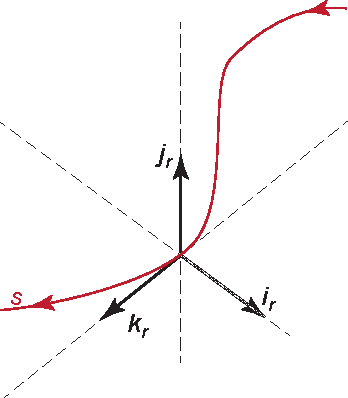
\includegraphics[width=0.80\linewidth]{RPLC.pdf}
  \end{center}
  \caption{
    Reference particle local coordinate system.
    The trajectory of the reference particle is shown as the red line.
    The distance the reference particle has travelled, measured from
    the origin of coordinates in the laboratory frame, is labelled
    $s$.
    The origin of the ``reference paricle local coordiante (RPLC)
    system is coincident with the position of the reference particle.
    The directions of unit vectors along each of three righthanded,
    orthogonal coordinate axes are shown as black arrows labelled
    $\bm{i}_r$, $\bm{j}_r$, and $\bm{j}_r$. 
  }
  \label{fig:RPLC}
\end{figure}

The trajectory of the reference particle is a straight line as it
traverses a drift space and a variety of beam-line elements.
Examples of such beam-line elements include solenoids and
quadrupoles.
The reference trajectory is also undeviated by passage through an
accelerating cavity placed such that the accelerating field is 
parallel to the reference-particle trajectory.

The RPLC coordinate system at $s=0$ is taken to coincide with the
laboratory coordinate system.
Beam-line elements are placed sequentially along the trajectory of the
reference particle.
If necessary a coordinate transformation is performed to ensure that
the RPLC system at the entrance to a particular beam-line element is
consistent with the definition given above.

\subsection{Transforming to and from reference particle local
            coordinates to laboratory coordinates}
            
In the RPLC system, the trajectory of the reference particle,
$\bm{R}_0$, is:
\begin{equation}
  \bm{R}_0(s) = \bm{0}\,.
\end{equation}
The position of a test particle in the RPLC frame, $\bm{R}$, is
described with reference to the position of the reference particle.
In the laboratory frame, the position of the test particle is:
\begin{equation}
  \bm{r}(s) = \bm{r}_0(s) + \bm{\delta r}(s) \,;
\end{equation}
where:
\begin{equation}
  \bm{\delta r}(s) = \underline{\underline{R}}(s) \bm{R}(s) \,{\rm ; and}
\end{equation}
$\underline{\underline{R}}(s)$ is a rotation matrix that takes
the RPLCs at $s$ to the laboratory frame coordinates.

In the laboratory frame, the unit vectors $\bm{i}_r$,
$\bm{j}_r$ and $\bm{k}_r$ are given by:
\begin{eqnarray}
  \bm{i}_r & = & \begin{pmatrix} i_{rx} \\ i_{ry} \\  i_{rz} \\ \end{pmatrix} \,;           \nonumber \\
  \bm{j}_r & = & \begin{pmatrix} j_{rx} \\ j_{ry} \\  j_{rz} \\ \end{pmatrix} \,{\rm ; and}           \\
  \bm{k}_r & = & \begin{pmatrix} k_{rx} \\ k_{ry} \\  k_{rz} \\ \end{pmatrix} \,.           \nonumber
\end{eqnarray}
The rotation matrix, $\underline{\underline{R}}$, may now be written:
\begin{equation}
  \underline{\underline{R}}(s) =
    \begin{bmatrix}
      i_{rx} & j_{rx} & k_{rx} \\
      i_{ry} & j_{ry} & k_{ry} \\
      i_{rz} & j_{rz} & k_{rz}
    \end{bmatrix} \,.
\end{equation}
